\chapter{An Overview of Scientific Visualization} % (fold)
\label{cha:sci_vis}
%
\lettrine[lines=3, findent=-2pt, nindent=4pt, loversize=0.02]{S}{cientific
visualization} is the visualization of data from the natural sciences.
%
Although such data can come in a variety of forms, the term is most often used
to describe the techniques used for displaying spatial, possibly time-varying
data from physics, chemistry, engineering, or biomedical applications.
%
Examples for such data are volumetric scans of patients from medicine, wind
speed and pressure measurements from meteorology, and simulations of the air
flow around a car.
%

%
This thesis presents several new scientific visualization techniques.
%
The techniques are applied to simulation data from two different engineering
domains: turbulent combustion and solid mechanics.
%
To set the scene for these contributions, we will therefore use this chapter to
give an overview of the most important methods for visualizing scientific data.
%
Such data usually comes in the form of scalar-, vector-, or (second-order)
tensor fields.
%
We will take a look at the definition and basic visualization techniques for
each of these types of fields in the following sections.
%

%
This chapter is necessarily sparse on details and omits a lot of basic knowledge
on computer graphics, data representation, numerical algorithms, and
visualization in general.
%
A more thorough introduction to the field is given in Alexandru Telea's book
``Data Visualization''~\cite{Telea2014}.
%
Material for further reading can be found in the references cited throughout the
text.
%
\section{Scalar Field Visualization} % (fold)
\label{sec:scalar_fields}
%
A scalar field is a map $s(\vx, t): D \times T \mapsto \RRSet$ that assigns a
scalar value to each position $\vx$ and time $t$ in spatial and temporal domains
$D$ and $T$.
%
The spatial domain $D$ is a subset of the (two- or three-dimensional) Euclidean
space $\EESet^n$.
%
The temporal domain $T$ is usually an interval of $\RRSet$.
%
Examples of scalar fields are the temperature in a solid object, the population
density on a map, and the attenuation coefficient in a \ac{CT} scan.
%
If the scalar field does not change with time, or we are only interested in a
single instant, we often just write $s(\vx)$ and omit the time parameter.
%

% \subsection{Visualization Methods for Scalar Fields} % (fold)
% \label{sub:visualization_methods_for_scalar_fields}
%
% \begin{itemize}
%     \item Space-filling
%     \begin{itemize}
%         \item Colormapping (2D)
%         \item Height-mapping (2D)
%         \item Direct Volume rendering (3D)
%     \end{itemize}
%     \item Geometry-based
%     \begin{itemize}
%         \item Isocontours/surfaces (cite marching cubes)
%         \item maxima/minima/saddles
%         \item Morse-Smale-complex
%         \item Ridge lines/surfaces
%     \end{itemize}
% \end{itemize}
%
Methods for visualizing scalar fields can be roughly separated into two groups:
image-based and geometry-based.
%
We will briefly cover the most important methods in the following.
%
\Todo{add citations}
%

\subsection{Image-Based Methods} % (fold)
\label{sub:scalar_image_based}
%
Image-based methods map the scalar at each position in space to a property and
display it directly.
%
Among such methods are \emph{color-mapping} and \emph{height-mapping} for
\ac{2D} scalar fields as well as \emph{direct volume rendering} for \ac{3D}
scalar fields.
%

%
\subsubsection{Color-Mapping}
%
Color-mapping means assigning each scalar value a color from a
predefined color map and displaying the result as an image or texture.
%
Due to its simplicity, it is probably the most widespread method presented here.
%
This technique is only applicable to \ac{2D} scalar fields, but is commonly used
on \ac{3D} data by selecting slices or surfaces in a volume, or by displaying
the scalar value on the outside surface of the volume.
%
\begin{figure}[t]
    % \centering
    \begin{captionbeside}{Direct volume rendering of a \ac{CT} scan of a human skull using
        volumetric raycasting with gradient-based shading. Image source: Wi\-ki\-me\-di\-a
        Com\-mons.\label{fig:direct_volume_rendering}}
        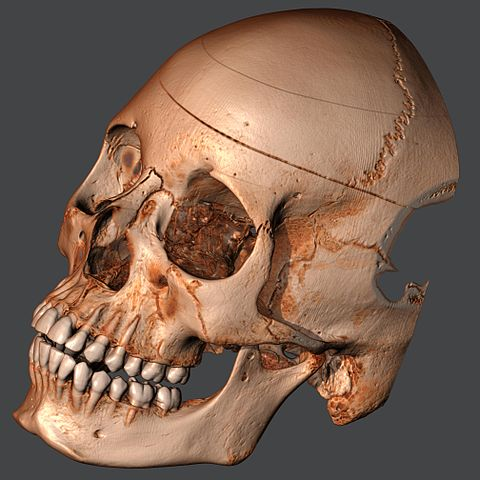
\includegraphics[width=0.6\textwidth]{figures/skull_direct_volume_rendering.jpg}
    \end{captionbeside}
\end{figure}
%

%
\subsubsection{Height-Mapping}
%
Height-mapping only works on \ac{2D} data.
%
It essentially means interpreting the scalar value at each point as a height
value and displaying the resulting three-dimensional surface.
%
Because it transforms \ac{2D} information into \ac{3D} information, it is best
suited for interactive settings, where the resulting surface can be rotated and
viewed from all directions.
%

%
\subsubsection{Direct Volume Rendering}
%
Direct volume rendering~\cite{Levoy1988,Drebin1988} is the extension of
color-mapping to \ac{3D} scalar fields.
%
It involves two steps: Applying a transfer function, and accumulating the
resulting colors and opacities along viewing rays to produce an image.
%
The transfer function has to be chosen carefully to reveal the structures in the
data that are interesting, and make the uninteresting parts transparent.
%
Color and opacity values are then accumulated along viewing rays to simulate the
transport of light through a semitransparent medium.
%

%
The shading of a solid surface can be approximated by using the gradient of the
scalar field as the surface normal (see \cref{fig:direct_volume_rendering}).
%
More advanced techniques use a two-dimensional transfer function that also takes
the gradient magnitude into account when deciding the color, opacity and
shading parameters of a point along the viewing ray~\cite{Kindlmann1998}.
%
% subsection scalar_image_based (end)

\subsection{Geometry-Based Methods} % (fold)
\label{sub:scalar_geometry_based}
%
Geometry-based methods extract some geometrical structures from the data and
display these structures.
%
\emph{Isocontours and -surfaces} belong in this category together with
topological features such as \emph{extremal- and saddle points}, as well as
\emph{ridge- and valley lines and -surfaces}.
%

%
\subsubsection{Isocontours and -surfaces}
%
Isocontours and -surfaces are subsets of the scalar field where the
scalar is equal to a constant (iso-) value.
%
In the literature these are also often referred to as \emph{level sets}.
%
They form lines or surfaces that are always closed or end at the domain
boundary, and that never intersect each other.
%
For \ac{2D} scalar fields, it is common to plot contours for several isovalues
at once, which resemble the height lines we know from maps.
%
In \ac{3D}, it is rare to display more than two or three different isosurfaces
at the same time due to occlusion problems.
%

%
\subsubsection{Critical Points}
%
Critical points are points in a scalar field where the gradient becomes zero.
%
As such, they are features of the scalar field's topology.
%
Critical points can be classified by the eigenvalues of the Hessian matrix at
the critical point:
%
If all eigenvalues are positive the point is a minimum, if all are negative it
is a maximum, and if the Hessian has both positive and negative eigenvalues,
the point is a saddle.
%

%
\subsubsection{Ridge- and Valley Lines and -Surfaces}
%
Ridge- and valley lines and -surfaces also belong to the category
of topological features.
%
There is no universal agreed-upon definition for these types of features.
%
The two most common, competing definitions are \emph{watersheds} and
\emph{height ridges}~\cite{Peikert2008,Eberly2012}.
%
Watersheds are global features that separate the scalar field into ``areas of
influence'' of the different minima (or maxima).
%
Imaginine a scalar field as a height field.
%
Starting a gradient descent from two points on the same side of a watershed
will end up in the same minimum.
%
Starting from two points on opposite sides of the watershed will end up in two
different minima.
%

%
Height ridges are defined by a local differential analysis of the scalar field.
%
As such, their computation is less costly, but they do not provide a
space-filling segmentation of the data.
%
Often, computation of raw ridges and valleys produces a lot of small and
insignificant features due to noise.
%
An additional filtering step~\cite{Peikert2008} can be applied to only keep the
most significant lines (see \cref{fig:ridge_valley_lines}).
%
\begin{figure}[t]
    \begin{captionbeside}
        {Filtered ridge and valley lines of a scalar field.
        Ridges are shown in red, valleys in blue. The scalar field is visualized
        using a combination of height mapping (to obtain the shading) and
        isocontours. Image source: Peikert and Sadlo~\cite{Peikert2008}.
        \label{fig:ridge_valley_lines}}
        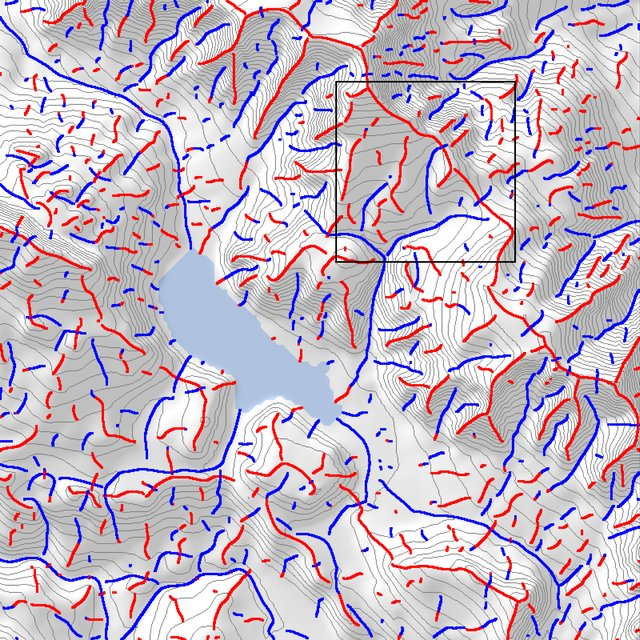
\includegraphics[width=0.6\textwidth]{figures/ridge_valley_lines_peikert.jpg}
    \end{captionbeside}
\end{figure}
%
\subsubsection{Morse-Smale Decomposition} % (fold)
\label{ssub:morse_smale_decomposition}
%
The Morse-Smale Decomposition forms the topological skeleton of a scalar field.
%
It is based on the idea of integral lines of the scalar field.
%
These are maximal paths that are everywhere tangent to the gradient of the
scalar field (see also integral curves in vector fields,
\cref{sub:integral_curves_and_surfaces}).
%
Integral lines always connect two critical points or end at the domain boundary.
%

%
The Morse-Smale decomposition separates the scalar field into a disjoint set of
cells whose union is the whole domain.
%
Each cell is defined as the set of all integral lines that connect the same
minimum and maximum.
%
In this sense, the Morse-Smale decomposition is closely related to the idea of
watersheds:
%
The boundarties of the cells are precisely the watersheds of the scalar field
and its negative.
%
% subsubsection morse_smale_decomposition (end)
%
% subsection scalar_geometry_based (end)
%
% subsection visualization_methods_for_scalar_fields (end)
%
% section scalar_fields (end)

\section{Vector Field Visualization} % (fold)
\label{sec:vector_fields}
%
A vector field $\vv(\vx,t): D \times T \mapsto \RRSet^n$ is a map from spatial
and temporal domains $D \subset \EESet^n$ and $T \subset \RRSet$ to the
$n$-dimensional vector space $\RRSet^n$.
%
Just like a scalar field, it assigns a value to each position and time in the
domains, but this time the value is a vector.
%
Examples for vector fields are the velocity of a fluid flow, the displacement
field of a deformed object, and the magnetic field around an electromagnet.
%
If the vector field does not change with time, or we are only interested in the
field at a single instant, we say that we have a \emph{steady} vector field
$\vv(\vx)$.
%
If the vector field changes with time, we call it an \emph{unsteady} vector
field.
%
If we are talking about a vector field representing the velocity of a fluid
flow, we sometimes call it a (steady or unsteady) \emph{flow field}.
%

%
Vector field visualization methods can be sorted into roughly six different
classes: Basic methods, image-based methods, integral curves and -surfaces,
topological features, vortex extraction and \acl{LCS}.
%
We will again visit the most important methods in the following sections.
%

%
\subsection{Basic Methods} % (fold)
\label{sub:vector_basic}
%
Basic methods display the vector data using simple techniques, much like
image-based methods for scalar fields.
%
They encompass techniques such as \emph{arrow plots}, or \emph{color-mapping}
the velocity magnitude, vorticity and other derived quantities directly.
%

%
\subsubsection{Arrow Plots}
%
Arrow plots are the simplest way to visualize a vector field.
%
In such a plot, arrow glyphs are placed at multiple locations throughout the
domain.
%
The arrows are aligned with the direction of the local vector, and their
length is typically scaled based on its magnitude.
%
Such plots can very accurately show the vectors at a limited number of
locations, but they quickly become cluttered once too many arrows are plotted,
or the arrows become too long and occlude each other.
%

%
\subsubsection{Color-Mapping}
%
Color-mapping can be applied to vector fields in different ways.
%
The most common one is simply displaying the magnitude of the vector field as a
scalar.
%
Other scalars derived from the vector field, such as the vorticity magnitude and
divergence, can be visualized in the same way.
%
All of this obviously goes along with a loss of information.
%
Since color has three degrees of freedom, a vector field can also be visualized
without information loss by directly mapping the vector values to colors.
%
The most naive way is to simply interpret the three components of a \ac{3D}
vector as RGB values.
%
Such images theoretically contain they full information of the original vector
field.
%
However, they are very hard to interpret, as there is no inherent meaningful
connection between the direction of the vector and the color it is mapped to.
%
This can be slightly improved for \ac{2D} vector fields by mapping the angle
and magnitude of the vector to hue and value of the HSV color space.
%
% subsection direct_methods (end)
%
\subsection{Image-Based Methods} % (fold)
\label{sub:vector_image_based}
%
Image-based methods visualize the vector data by generating a space-filling
texture.
%
Among such methods are \emph{line integral convolution}, \emph{spot noise},
and \emph{texture advection}.
%

%
\subsubsection{Line Integral Convolution}
%
Line integral convolution (\acs{LIC}\acused{LIC})\cite{Cabral1993} is the most
popular image-based vector field visualization method.
%
It is based on ``smearing'' a random noise texture along stream lines of a
\ac{2D} vector field.
%
More specifically, the color at a certain position is determined as a weighted
integral of the color values encountered along a stream line passing through
that position.
%
The result is a space-filling image where the direction of the vector field is
visible at each location (see \cref{fig:lic_topo}).
%
The basic \ac{LIC} technique is only applicable to \ac{2D} steady vector fields,
but extensions have been developed for \ac{3D}~\cite{Rezk-Salama1999} and
unsteady~\cite{Shen1997} datasets.
%

%
\subsubsection{Spot Noise}
%
Spot noise is also a method designed for \ac{2D} data and produces results
similar to \ac{LIC}~\cite{Wijk1991,Leeuw1995}.
%
It works by blending noise sprites that have been stretched and rotated
according to the local vector direction.
%
In contrast to \ac{LIC}, spot noise better represents the local vector
magnitude, but in regions with low magnitude, the vector direction is not well
visible.
%

%
\subsubsection{Texture Advection}
%
Texture advection works on \ac{2D} steady and unsteady vector fields.
%
It is best suited for vector fields representing a flow, as it simulates the
transport(advection) of a texture with the flow.
%
A texture is placed in the flow at some point in time, and each point on the
texture is moved with the flow over time.
%
As time progresses, the texture is warped, and the viewer can follow where each
part of the texture is transported.
%
This method has a lot in common with the integration-based methods presented in
the next section.
%
In fact, texture advection simply displays a time surface with a mapped texture
in a \ac{2D} vector field.
%

%
% subsection vector_image_based (end)
%
\subsection{Integral Curves and -Surfaces} % (fold)
\label{sub:integral_curves_and_surfaces}
%
Integral curves and -surfaces are generated by integrating the vector field
starting from different kinds of seed structures.
%
Depending on the seeding strategy and the kind of vector field, we can obtain
\emph{streamlines}, \emph{pathlines}, \emph{streaklines}, \emph{timelines},
and the accompanying surfaces\ToCite{Batchelor}.
%
Since integral structures play an important role in several parts of this
thesis, we will cover them here in more detail.
%
\begin{figure}[t]
    \centering
    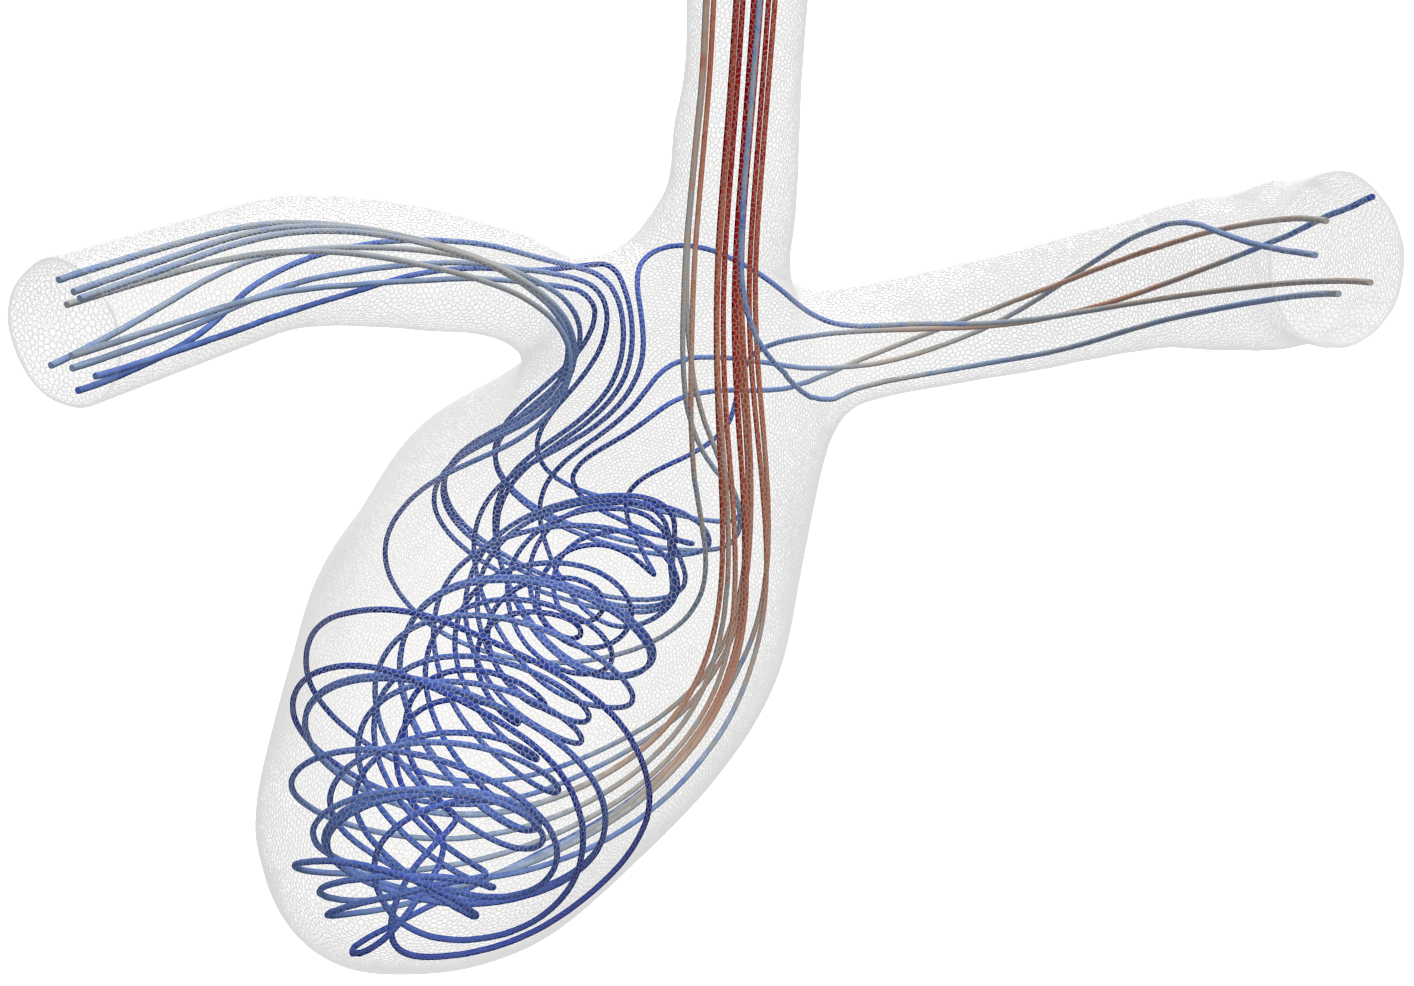
\includegraphics[width=0.9\textwidth]{figures/pathlines_aneurysm.png}
    \caption{Streamlines in the simulated flow through a cranial aneurysm.
             Image courtesy of Tim Gerrits~\cite{Gerrits2018}.}
    \label{fig:streamlines}
\end{figure}
%

\subsubsection{Streamlines} % (fold)
\label{ssub:streamlines}
%
Streamlines are the simplest form of integral curve in a vector field.
%
They are defined for steady vector fields.
%
Depending on the application area, they are also sometimes called \emph{field
lines}.
%
A streamline is a curve that is tangent to the vector field everywhere along its
path.
%
Given a streamline $\vc(s)$ of the steady vector field $\vv(\vx)$, this means
that $\vc(s) \times \vv(\vc(s))$ is $\vNull$ for all $s$.
%
This criterion is valid for any parameterization of the curve, but we can only
use it to check if a given curve is a streamline.
%
To compute streamlines, we typically solve the ordinary differential equation
%
\begin{equation*}
    \frac{\partial \vc(s)}{\partial s} = \vv(\vc(s))
    \text{, with } \vc(0) = \vx_0 \, \text{.}
\end{equation*}
%
This yields a streamline with a particular parameterization: an integral curve
of the vector field.
%
Due to their definition, two stream lines never intersect at single points.
%
They are either completely disjoint, or they coincide.
%

%
Visualizing a steady vector field with stream lines shows the direction of the
flow much like a \ac{LIC} image does, but not in a space-filling manner.
%
This allows for use of streamlines also in \ac{3D} data (see
\cref{fig:streamlines}).
%
Streamline visualization can be deceiving when used on single time slices of
an unsteady flow field.
%
The connected lines mistakenly suggest paths of fluid elements.
%
However, if the flow field changes significantly with time, the actual paths of
fluid elements can deviate significantly from the streamlines in a single time
slice.
%
In this case, the more appropriate visualization tools are pathlines,
streaklines, and timelines, which incorporate the temporal information of the
flow.
%
% subsubsection streamlines (end)

\subsubsection{Pathlines} % (fold)
\label{ssub:pathlines}
%
Pathlines describe the paths of massless particles moving with a
flow.
%
They are defined as the solution to the ordinary differential equation
%
\begin{equation*}
    \frac{\partial \vc(t)}{\partial t} = \vv(\vc(t), t)
    \text{, with } \vc(t_0) = \vx_0 \, \text{,}
\end{equation*}
%
where $\vc(t)$ is the curve of the pathline, $t$ is time, and $\vv(\vx, t)$ is
an unsteady vector field.
%
Looking at this definition, it becomes apparent that for a steady vector field,
which does not change with time, streamlines and pathlines are identical.
%

%
The set of all pathlines for all possible combinations of start position
$\vx$, start time $t_0$ and end time $t$ forms the \emph{flow map}.
%
This function, which we write as $\bPhi(\vx, t_0, t)$, determines where a
massless particle starting at position $\vx$ and time $t_0$ ends up after
advecting with the flow until time $t$.
%

%
Pathlines allow the visualization of the dynamic behavior of an unsteady flow
in a static image.
%
To show the temporal information, the time is often color-mapped on the curve.
%
Unlike streamlines, pathlines can and do intersect each other.
%
For very complex flows, showing a lot of pathlines can therefore quickly become
confusing.
%
In such cases it can be better to show animated streaklines instead.
%
% subsubsection pathlines (end)

\subsubsection{Streaklines} % (fold)
\label{ssub:streaklines}
%
Streaklines are the connected locations of a continuously injected
stream of massless particles into a flow.
%
They approximate the behavior of a thin stream of dye injected at a certain
position that is often applied in experimental settings to visualize the flow.
%
Formally, a streakline is formed by the connected endpoints of a set of
pathlines with the same start position and end time, but continuously increasing
start time.
%
Using the flow map $\bPhi$, which we introduced earlier, we can formally define
a streakline as
%
\begin{equation*}
    \vc(s) = \bPhi(\vx, s, t)\,\text{,}
\end{equation*}
%
where $t$ is the current time, $\vx$ is the injection point, and $s$ is the
continuously increasing start time that runs along the curve.
%
Like pathlines, streaklines also become identical to streamlines if the flow
does not change with time.
%

%
While a pathline shows the behavior of the flow over a period of time, a
streakline only ever shows the position of the injected particles at a
single time instant.
%
Streaklines are therefore often animated by continuously increasing the end
time $t$ and injecting more particles.
%
This again mirrors the behavior of injected dye observed in an experiment.
%
% subsubsection streaklines (end)

\subsubsection{Timelines} % (fold)
\label{ssub:timelines}
%
Timelines are different from all the previous integral lines in that
their seeding structure is not a single point, but a whole line.
%
A timeline is formed by placing a line somewhere in the flow, treating it as a
set of massless particles, and letting the whole line advect with the flow at
once.
%
Formally, a time line is formed by the connected endpoints of a set of pathlines
with the same start and end time, but continuously changing start position.
%
Given a seed curve $\vs(s)$ and start and end times $t_0$ and $t$, we can
formally define a timeline in terms of the flow map as
%
\begin{equation*}
    \vc(s) = \bPhi(\vs(s), t_0, t)\,\text{.}
\end{equation*}
%
Much like streaklines, timelines are often animated to show the progressive
effect of the flow.
%
As the end time $t$ advances, the line is transported and warped by the flow and
visualizes the way the flow mixes and perturbs a region of the fluid.
%
\begin{figure}[t]
    \centering
    \MissingFigure{Image illustrating relationship between pathlines,
    streaklines and timelines}
    \caption{Pathlines, streaklines and timelines of a \ac{2D} vector field.}
    \label{fig:path_streak_timelines}
\end{figure}
%
% subsubsection timelines (end)

\subsubsection{Integral Surfaces} % (fold)
\label{ssub:integral_surfaces}
%
Integral surfaces can be formed from any of the integral lines by using a
higher-dimensional seeding structure.
%
For stream-, path-, and streaklines this means using a line as the seeding
structure.
%
Timesurfaces are formed by using a surface as the seed.
%
Integral surfaces can be helpful for visualization because they have a better
visual coherency than a number of single lines.
%
The curvature, wrinkling and folding of structures induced by the flow become
easier to grasp when using integral surfaces.
%
On the flip side, integral surfaces have more of a problem with occlusion
compared to lines, as they are more massive.
%
% subsubsection integral_surfaces (end)

%
% subsection integral_lines_and_surfaces (end)
%
\subsection{Vector Field Topology} % (fold)
\label{sub:vector_field_topology}
%
% The topology of a vector field is defined by \emph{critical points},
% \emph{boundary switch points/lines}, \emph{attachment- and detachment
% points/lines}, the accompanying \emph{separatrices} connecting these points,
% and \emph{isolated closed streamlines}.
%
The topology of a vector field is defined by \emph{critical points},
\emph{separation- and attachment points} and the accompanying
\emph{separatrices} connecting them.
%
Together, they form a sort of skeleton of the vector field, from which the
behavior of the full field can be inferred.
%
\begin{figure}[t]
    % \centering
    \begin{captionbeside}
        {\ac{LIC} of a \ac{2D} vector field with overlaid vector field topology
        consisting of critical points, boundary switch points, and separatrices.
        Image source: Holger Theisel.\label{fig:lic_topo}}
        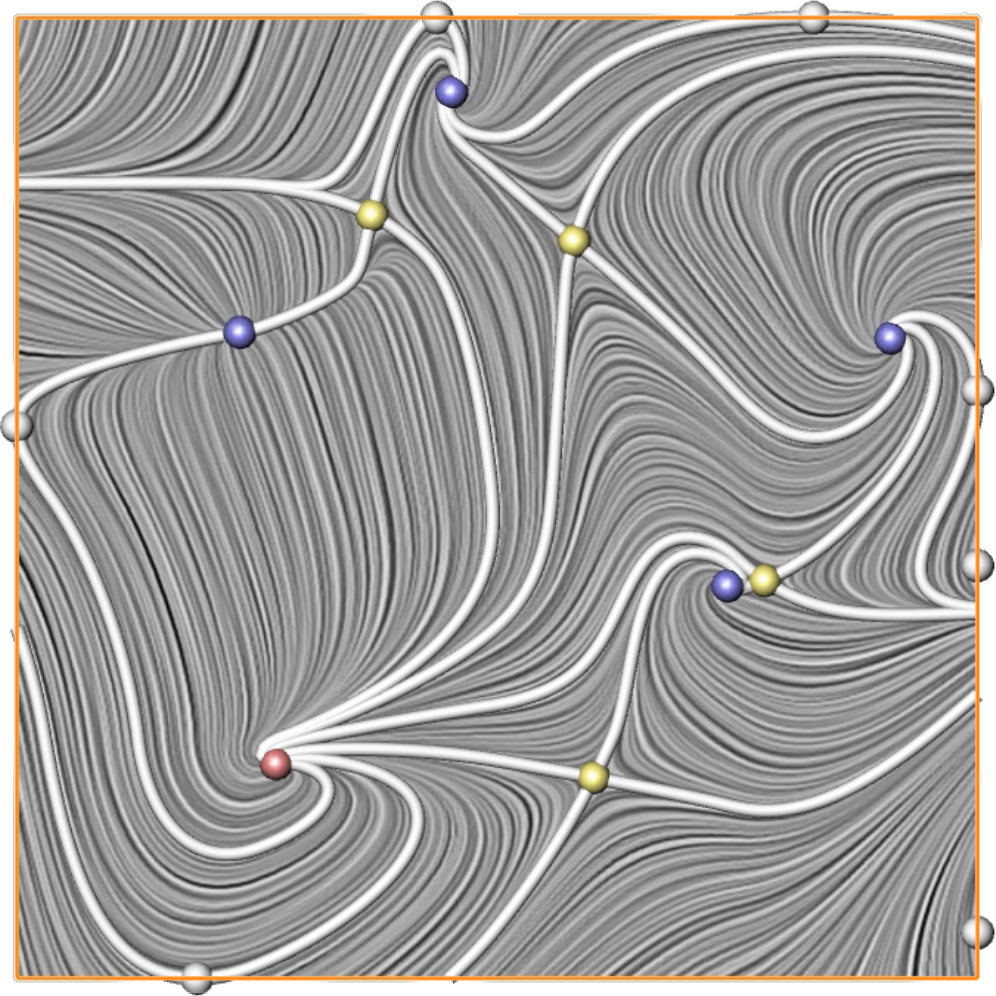
\includegraphics[width=0.6\textwidth]{figures/lic_topology.png}
    \end{captionbeside}
\end{figure}
%

\subsubsection{Critical Points} % (fold)
\label{ssub:critical_points}
%
Critical points of a vector field are locations where the magnitude
of the vector becomes zero.
%
They are interesting because they are at the centers of interesting structures
in the vector field.
%
Critical points in vector fields can be sorted into different categories.
%
Which category a critical point belongs to depends on the behavior of the vector
field in its vicinity, which is encoded in its derivative.
%
The Jacobian matrix $\mJ(\vv) = \vv \T{\nabla}$ gathers the partial derivatives
of all components of the vector field.
%
The signs of the real parts of its eigenvalues indicate if the vector field is
attracting or repelling in the vicinity of the critical point.
%
Depending on these signs, the critical point can be categorized into
\emph{sinks} (negative), \emph{sources} (positive), and \emph{saddles} (mixed
signs).
%
The presence of an imaginary part of the eigenvalues/eigenvectors indicates
swirling behavior.
%
A more in-depth discussion of critical points in vector fields has been provided
by Helman and Hesselink~\cite{Helman1991}.
%
% subsubsection critical_points (end)

%
% \paragraph{Boundary switch points/lines} are locations where the vector field
% is parallel to the boundary of the domain.
% %
% They separate inflow and outflow boundary regions.
% %

\subsubsection{Separation- and Attachment Lines/Surfaces} % (fold)
\label{ssub:separation_attachment_lines}
%
Separation- and attachment lines/surfaces occur on no-slip boundaries.
%
They are locations where the flow separates from/attaches to a surface.
%
In a \ac{2D} flow, these are points.
%
In \ac{3D}, they can be point or line structures.
%
Separation- and attachment structures are similar to critical points of the
vector field, specifically to saddles, in that they are end points of
streamlines of the vector field.
%
However, they are not exactly critical points, as the velocity is zero
everywhere on a no-slip boundary.
%
Instead, they are topological features of the skin friction field, which
describes the shear of the flow near the boundary~\cite{Surana2006}.
%
% subsubsection separation_attachment_lines (end)

\subsubsection{Separatrices} % (fold)
\label{ssub:separatrices}
%
Separatrices connect critical points with each other.
%
They are lines in \ac{2D} vector fields and can be lines or surfaces in \ac{3D}
vector fields~\cite{Helman1989,Helman1991}.
%
Separatrices start at saddle points or separation-/attachment points.
%
They are streamlines with a special property: Streamlines passing through two
points on opposite sides of the separatrix will diverge from each other near a
saddle or separation-/attachment point in forward or backward flow direction.
%
As such, they separate the flow into distinct regions that streamlines starting
in these regions will never leave.
%
Because streamlines and separatrices are an instantaneous observation (they
exist in steady vector fields or at single points in time in an unsteady vector
field), this does not imply that pathlines will never leave these regions in
unsteady flow.
%
For unsteady flows, the equivalent of separatrices are \acl{LCS}, which we will
cover in the next section.
%
% subsubsection separatrices (end)
%
% subsection vector_field_topology (end)
%
\subsection{Vortex Extraction} % (fold)
\label{sub:vortex_extraction}
%
Vortices are structures in a flow that show a swirling motion around a common
center.
%
They will usually stay intact for long periods of time.
%
Vortices are the defining characteristic of turbulent flow.
%
The study of their behavior is a central topic of current fluid dynamics
research.
%
Even though the concept of a vortex seems rather simple, hundreds of years of
fluid dynamics research still has not resulted in a universally accepted formal
definition.
%
This is why there is a plethora of methods for detecting and quantifying
vortices in the literature.
%
Most methods can be sorted into two categories: \emph{region-based} and
\emph{line-based}.
%
They can be further classified by their invariance to transformations of the
reference frame through which the flow is observed.
%
Non-invariant methods are sensitive to all reference frame transformations.
%
Galilean invariant methods are insensitive to any motion of the reference frame
with constant speed and direction.
%
Objective methods are insensitive to any smooth translation and rotation of the
reference frame.
%
We will cover some significant vortex extraction methods here.
%
An extensive survey on the subject has been done by G\"unther and
Theisel~\cite{Guenther2018}.
%

%
Region-based methods measure the ``vortex-ness'' of the flow at a point by a
scalar quantity.
%
Applying a threshold to this quantity shows the vortex regions.
%
Notable representatives of this category are the \emph{vorticity magnitude},
\emph{$\lambda_2$-criterion} and \emph{Q-criterion}, which are all Galilean
invariant methods that work on steady vector fields.
%
Recently, the \emph{\acl{IVD}}~(\acs{IVD}) has been proposed as an objective
criterion for steady vector fields.
%
Its extension, the \emph{\acl{LAVD}}~(\acs{LAVD}) also accounts for unsteady
behavior of the flow.
%
Region-based approaches are generally simple and efficient to implement, but the
results are dependent on the choice of the threshold, and they do not produce
explicit representations of the vortices.
%

%
Line-based methods explicitly extract the vortex core line that is the center
of the swirling behavior.
%
The \emph{reduced velocity} approach for extracting vortex core lines in steady
flows was proposed by Sujudi and Haimes~\cite{Sujudi1995} and later identified
as an application of the \emph{parallel vectors} operator by Peikert and
Roth~\cite{Peikert1999}.
%
This approach is only Galilean invariant when applying it to \ac{2D} vector
fields.
%
A Galilean invariant approach for finding the \emph{cores of swirling particle
motion} in unsteady flows was proposed by Weinkauf \etal \cite{Weinkauf2007}.
%
Recently, G\"unther \etal~\cite{Guenther2017} provided a framework for
objective vortex core detection.
%
This is realized by determining a locally \emph{near-steady frame} for observing
the flow.
%
\begin{figure}[t]
    \centering
    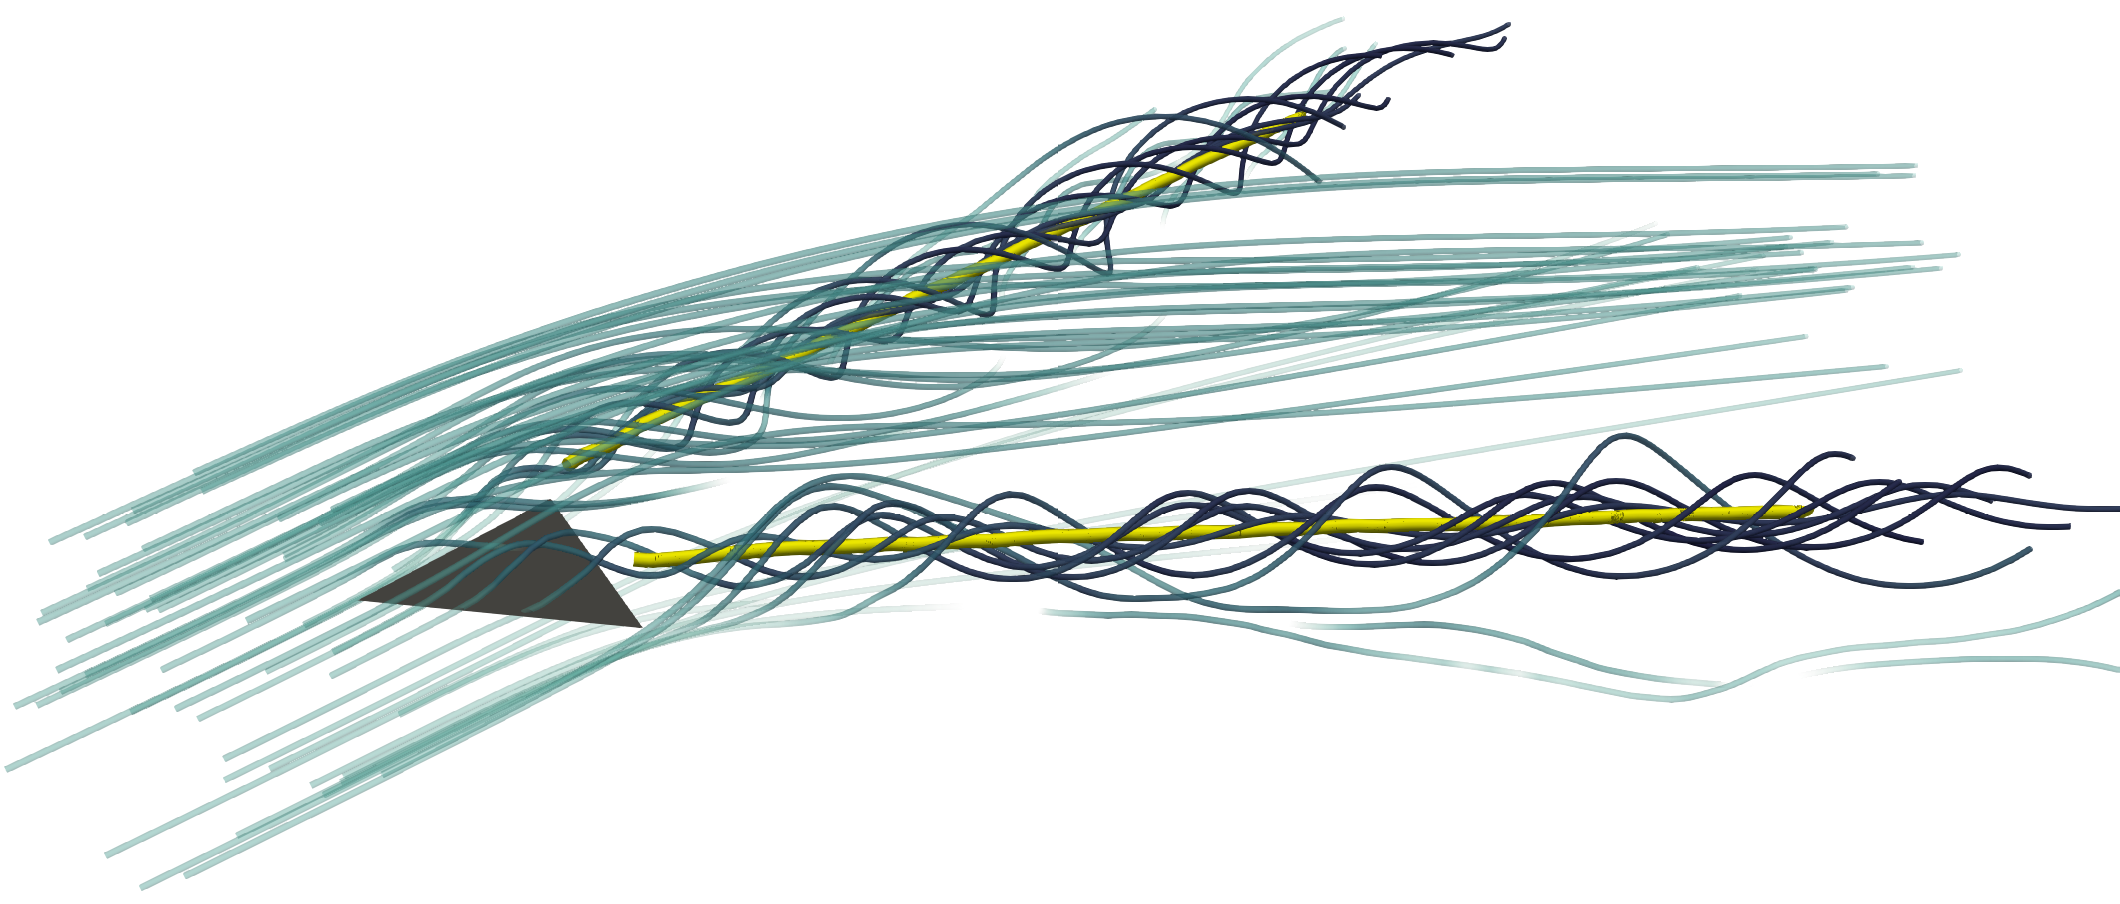
\includegraphics[width=\linewidth]{figures/DeltaWingStreamlines.png}
    \caption{Vortex core lines (yellow) and streamlines (blue) in the steady
    flow around a delta wing.}
    \label{fig:delta_wing_vortex_cores}
\end{figure}
%

%
\subsubsection{Vorticity Magnitude} % (fold)
\label{ssub:vorticity_magnitude}
%
The vorticity is commonly used in fluid dynamics literature to characterize the
rotational behavior of the flow.
%
It is defined as the curl of the flow field $\nabla \times \vv$.
%
The result is a vector field that points in the direction of the local axis of
rotation and whose magnitude indicates the rotation strength.
%
Vorticity magnitude is sometimes used to detect vortices.
%
However, a constant threshold over the whole domain is often not sufficient to
detect and distinguish all vortices, and it might yield false-positives in shear
flow.
%
This is why other methods often perform better.
%
% subsubsection vorticity_magnitude (end)
%
\subsubsection{Q-Criterion} % (fold)
\label{ssub:q_criterion}
%
The Jacobian $\mJ$ of a flow field can be decomposed into a symmetric part $\mS$
(often called \emph{strain rate tensor}) and an asymmetric part $\bOmega$ (often
called \emph{vorticity tensor}) where
%
\begin{equation*}
    \mS = \frac{\mJ + \T{\mJ}}{2}\text{,}\quad
    \bOmega = \frac{\mJ-\T{\mJ}}{2}\text{.}
\end{equation*}
%
For divergence-free (\ie, incompressible) flows, the Q-criterion states that a
region belongs to a vortex if the vorticity tensor is stronger than the strain
rate tensor, \ie,
%
\begin{equation*}
    (\Norm{\bOmega}^2 - \Norm{\mS}^2) > 0 \, \text{.}
\end{equation*}
%
The resulting regions are not as sensitive to the scaling of the data as the
vorticity magnitude.
%
% subsubsection q_criterion (end)
%
\subsubsection{$\bm{\lambda_2}$-Criterion} % (fold)
\label{ssub:lambda_2}
%
The $\lambda_2$-criterion~\cite{Jeong1995} uses invariants of the Jacobian to
detect pressure valleys in incompressible flows.
%
It identifies vortex core regions by investigating the eigenvalues of the tensor
$\mS^2+\bOmega^2$.
%
If the local tensor has at least two negative eigenvalues (\ie, if the middle
eigenvalue $\lambda_2$ is smaller than zero), a point is considered to belong to
a vortex core region.
%
In most cases, $\lambda_2$-criterion and Q-criterion yield similar results.
%
% subsubsection lambda_2 (end)
%
\subsubsection{\acs{IVD}/\acs{LAVD}} % (fold)
\label{ssub:ivd_lavd}
%
Recently, Haller \etal~\cite{Haller2016} proposed the \acf{IVD} as an objective
vortex measure for steady flow fields.
%
It is based on the observation that while the vorticity itself is not objective,
the difference between two vorticity vectors is.
%
Based on this, they define the \ac{IVD} as the difference of the local vorticity
to the average vorticity in a local neighborhood.
%
The \ac{LAVD} extends this to unsteady flows by integrating the \ac{IVD} along
a pathline over a certain time interval.
%
% subsubsection ivd_lavd (end)
%
\subsubsection{Reduced Velocity/Parallel Vectors} % (fold)
\label{ssub:reduced_velocity_parallel_vectors}
%
The first line-based method we present here was proposed by Sujudi and
Haimes~\cite{Sujudi1995} and works on steady flow fields.
%
It is based on the observation that vortex centers look like critical points
when looking at a slice of the vector field that is orthogonal to the vortex
core line.
%
In regions with swirling flow, the Jacobian has two complex conjugate and one
real eigenvector, which points along the local axis of rotation.
%
The reduced velocity or Sujudi/Haimes criterion therefore states that a vortex
core line is located where the projection of the local velocity onto a plane
orthogonal to the single real eigenvector is zero.
%
Peikert and Roth~\cite{Peikert1999} later discovered that this is equivalent to
locations where the velocity vector $\vv$ is parallel to its acceleration
$\mJ\vv$, and so is an application of the \emph{parallel vectors} operator,
which does not require the explicit computation of eigenvectors.
%
% subsubsection reduced_velocity_parallel_vectors (end)
%
\subsubsection{Cores of Swirling Particle Motion} % (fold)
\label{ssub:cores_of_swirling_particle_motion}
%
The method of Sujudi/Haimes only considers steady flow fields, or instantaneous
snapshots of unsteady flows.
%
This means that this method finds the centers of swirling streamlines.
%
In unsteady flows, streamlines and pathlines appear to swirl around different
cores if the vortex moves over time (see
\cref{fig:cores_of_swirling_particle_motion}).
%
Weinkauf \etal~\cite{Weinkauf2007} therefore developed an approach to find the
cores of swirling pathlines in unsteady flows.
%
They express pathlines as streamlines in a flow field with one more dimension
where time has been included as an additional explicit state variable.
%
For \ac{3D} unsteady flows, the pathlines are streamlines in \ac{4D} space-time.
%
They derive a criterion similar to Sujudi/Haimes for \ac{4D} vector fields that
can be reduced to a parallel vectors operation on two derived \ac{3D} vector
fields.
%
\begin{figure}[t]
    \centering
    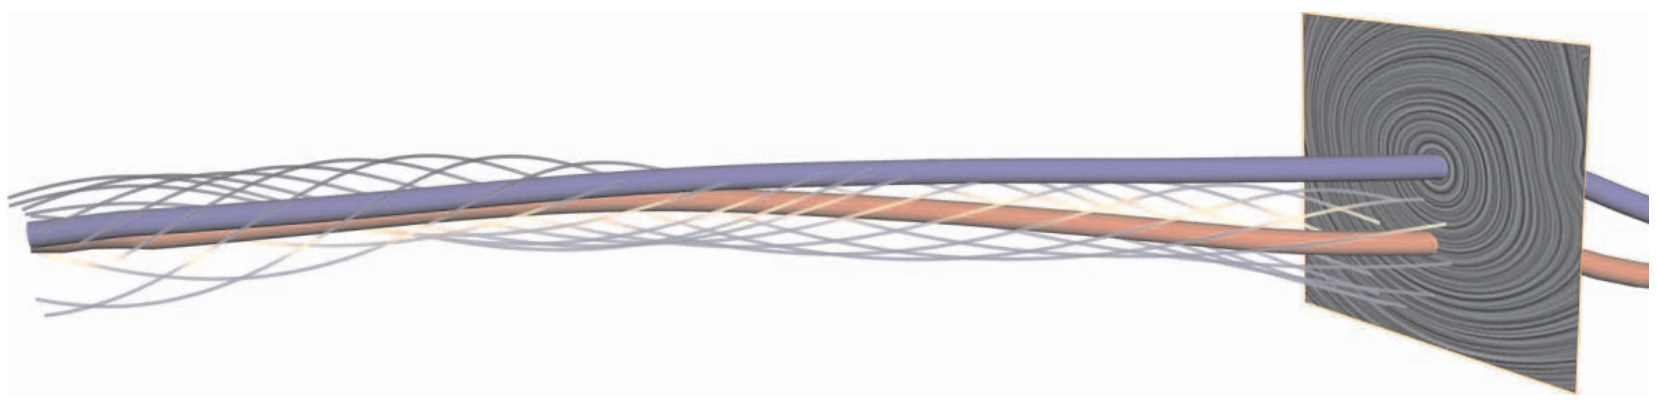
\includegraphics[width=\textwidth]{figures/pathline_streamline_core.png}
    \caption{Streamlines and pathlines swirl around different cores. The red
    tube shows the core of pathlines of a \ac{2D} vector field (rendered in
    \ac{3D} spacetime). The blue tube shows the path of the vortex core
    extracted from the individual time slices. Source: Weinkauf
    \etal~\cite{Weinkauf2007}.}
    \label{fig:cores_of_swirling_particle_motion}
\end{figure}
%
% subsubsection cores_of_swirling_particle_motion (end)
%
\subsubsection{Near-Steady Frame} % (fold)
\label{ssub:near_steady_frame}
%
The optimal reference frame for observing a vortex is a frame that follows the
vortex center over time~\cite{Robinson1991}.
%
In such a frame, the observed vector field around the vortex becomes almost
steady as ambient effects of larger flow structures are eliminated.
%
This is the basis of the approach proposed by G\"unther
\etal~\cite{Guenther2017}.
%
For each point in the flow, a locally optimal reference frame is computed in
which the flow becomes almost steady.
%
The reference frame is determined for a finite-sized neighborhood via a simple
linear optimization.
%
Once the vector field (and its derivatives) have been ``objectified'', any
region- or line-based vortex extractor that is designed for steady vector fields
can be used to extract objective unsteady vortices.
%
% subsubsection near_steady_frame (end)
%
% subsection vortices (end)
%
\subsection{Lagrangian Coherent Structures} % (fold)
\label{sub:lagrangian_coherent_structures}
%
\acf{LCS} are structures that show a locally maximal attracting or repelling
behavior of massless particles.
%
As the name suggests, these structures also tend to stay coherent over longer
time periods.
%
They can be thought of as a counterpart to vortices.
%
Whereas vortices represent the centers of swirling behavior, \ac{LCS} tend to
be located at the boundaries between vortices.
%
They act as transport barriers that have a minimal transverse flux of material
and are therefore very important for the investigation of mixing and transport
processes.
%
There are a number of very different methods for the investigation of \ac{LCS}.
%
A survey and comparison of some notable methods can be found
in~\cite{Hadjighasem2017}.
%

%
One popular approach to detecting \ac{LCS} is the investigation of the local
Lyapunov exponent~\cite{Ott2002}.
%
The Lyapunov exponent describes the rate of separation of infinitesimally close
trajectories over an infinite time interval.
%
Since real-world data is usually finite in time and space, two approximations of
the Lyapunov exponent are commonly used in practice: the
\emph{\acl{FTLE}\acused{FTLE}} (\acs{FTLE})~\cite{Haller2001} and
\emph{\acl{FSLE}\acused{FSLE}} (\acs{FSLE})~\cite{Aurell1997}.
%
It has been shown that ridges of the \ac{FTLE} or \ac{FSLE} field correspond
well to the locations of \ac{LCS}~\cite{Shadden2005,Haller2001}.
%

%
The basis for the computation of both \ac{FTLE} and \ac{FSLE} is the right
Cauchy-Green deformation tensor
%
\begin{equation*}
    \mC(\vx, t_0, t) = \T{\mF(\vx, t_0, t)}\, \mF(\vx, t_0, t) \,\text{,}
\end{equation*}
%
where $\mF$ is the deformation gradient obtained from the derivative of the
flow map
%
\begin{equation*}
    \mF(\vx, t_0, t) = \bPhi(\vx, t_0, t)\T{\nabla}\text{.}
\end{equation*}
%
The Cauchy-Green tensor describes the deformation the infinitesimal neighborhood
of a point $\vx$ at time $t_0$ experiences when advecting with the flow until
time $t$.
%
The maximum eigenvalue $\lambda_{\text{max}}$ of this tensor is a measure for
the maximum separation of two particles starting in this infinitesimal
neighborhood.
%
\subsubsection{Finite-Time Lyapunov Exponent} % (fold)
\label{ssub:ftle}
%
The \acl{FTLE} measures the maximum separation of neighboring particles after
advecting with the flow for a finite time:
%
\begin{equation*}
    \text{FTLE}(\vx, t_0, \tau)
        = \frac{1}{|\tau|}
          \ln\sqrt{\lambda_{\max}\left[\mC(\vx, t_0, t_0 + \tau)\right]}\,\text{.}
\end{equation*}
%

%
A straightforward way of approximating the \ac{FTLE} of a flow is to compute the
flow map $\bPhi$ on a discrete grid and estimate the deformation gradient $\mF$
via central differences.
%
Since the ridges of an \ac{FTLE} field can become very sharp with increasing
time interval $\tau$, this is usually not very accurate.
%
Additionally, we are usually not interested in an accurate estimation of regions
without ridges.
%
For this reason, there are multiple numerical schemes for more precise or
performant \ac{FTLE} computations.
%
A good overview of the existing methods is provided in Alexander Kuhn's PhD
thesis~\cite{Kuhn2013}.
%
\begin{figure}[t]
    \centering
    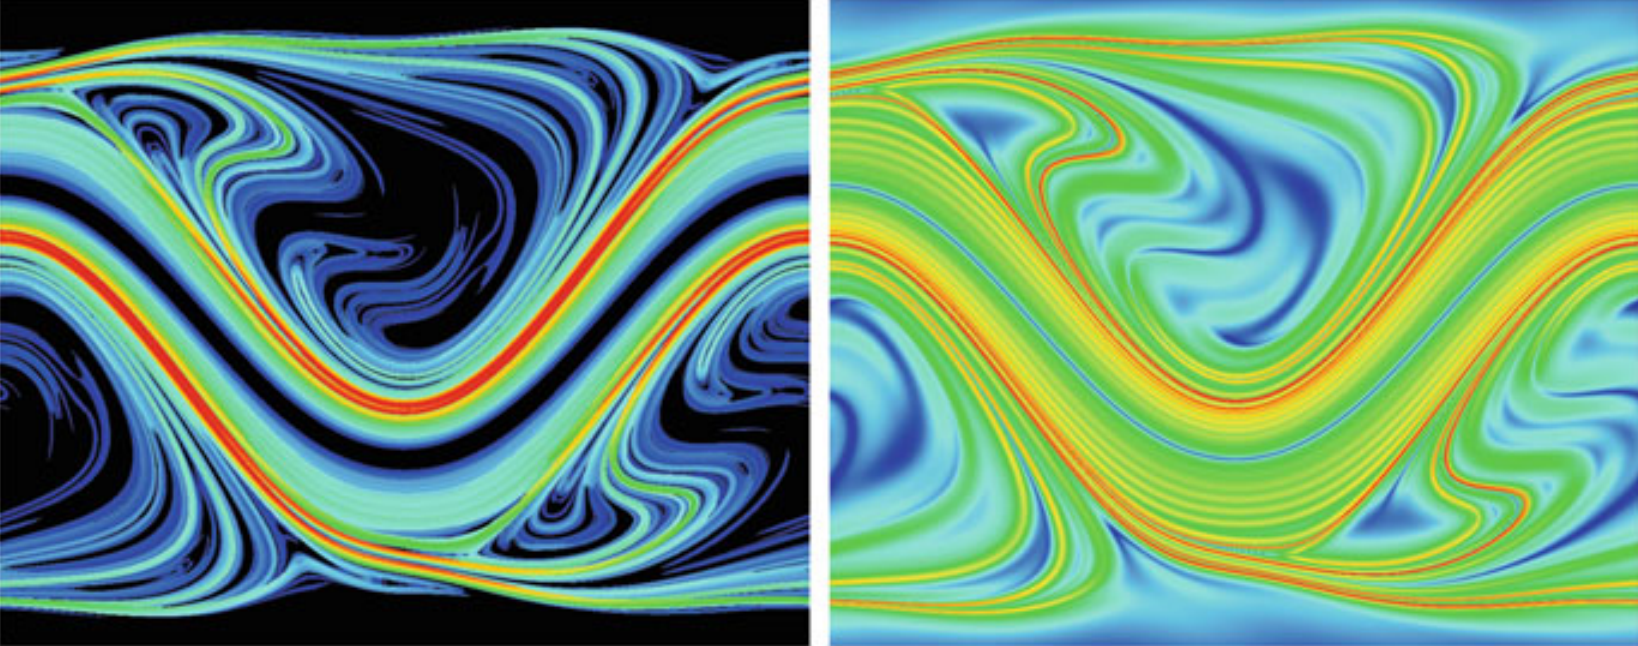
\includegraphics[width=\textwidth]{figures/fsle_ftle_peikert.png}
    \caption{Comparison of \ac{FSLE} (left) and \ac{FTLE} (right) of the flow
    field of a meandering jet. Image source: Peikert \etal~\cite{Peikert2014}.}
    \label{fig:ftle_fsle}
\end{figure}
%
% subsubsection ftle (end)
%
\subsubsection{Finite-Size Lyapunov Exponent} % (fold)
\label{ssub:fsle}
%
The \acl{FSLE} measures the time a pair of infinitesimally close particles
need to separate by a constant amount in space:
%
\begin{equation*}
    \text{FSLE}(\vx, t_0, r) = \frac{1}{|\tau_r|} \ln{r}\,\text{,}
\end{equation*}
%
where $\tau_r$ is the minimum time interval for which
%
\begin{equation*}
    \sqrt{\lambda_{\max}\left[\mC(\vx, t_0, t_0+\tau_r)\right]} = r\,\text{.}
\end{equation*}
%

%
\ac{FSLE} is popular in the oceanography community, but has not been adopted
much in the general visualization community.
%
As a result, \ac{FSLE} computation schemes in the literature are mostly
straightforward.
%
Either the maximum separation $\lambda_{\text{max}}$ is estimated by a discrete
sampling of the flow map in different
directions~\cite{dOvidio2004,Hernandez-Carrasco2011}, or the Cauchy-Green tensor
is estimated based on central differences~\cite{Peikert2014}.
%

%
\ac{FTLE} and \ac{FSLE} yield similar results, given the right parameters (see
\cref{fig:ftle_fsle}).
%
However, their semantic differences might make one or the other more appropriate
depending on the application.
%
While \ac{FTLE} operates on a finite integration time $\tau$, which must be
estimated a-priori, it shows the behavior of the flow for all scales of spatial
separation.
%
In contrast, \ac{FSLE} needs the choice of a separation size, which might be
more intuitive.
%
It yields information about separation at different spatial scales, but it does
not show separation that is smaller than the given threshold $r$.
%
% subsubsection fsle (end)
%
% subsection lagrangian_coherent_structures (end)
%
% section vector_fields (end)
%
\section{Second-Order Tensor Field Visualization} % (fold)
\label{sec:tensor_fields}
%
Although tensors are a very general concept in mathematics, when we talk about
tensor fields in scientific visualization, we generally mean a map $\mT(\vx, t):
D \times T \mapsto \RRSet^{m \times m}$ from spatial domain $D \in \EESet^n$ and
temporal domain $T \in \RRSet$ to the space of second-order tensors which can be
represented by matrices from $\RRSet^{m \times m}$.
%
While a vector describes an effect acting on a point, a second-order tensor
describes an effect on a vector.
%
Often, this means that the tensor describes some sort of differential effect
that acts on the infinitesimal neighborhood of a point.
%
Second-order tensor fields occur in a variety of different scientific contexts.
%
Some examples are stress and strain tensors in mechanical engineering
applications, and diffusion tensors occurring in \ac{DTI}, a special \ac{MRI}
modality used to visualize fiber tracts, \eg, in the human brain.
%
In reality, these tensor fields vary in time.
%
However, in practice datasets with temporally varying tensor fields are
relatively rare, and visualization methods are mostly designed for instantaneous
tensor fields $\mT(\vx)$.
%

%
The most important tensor field visualization methods can be roughly classified
into five different categories:
%
direct, image-based, glyph-based, line-/surface-based and topology-based.
%

\subsection{Direct Methods} % (fold)
\label{sub:tensor_direct_methods}
%
Direct methods display some properties of the tensor directly.
%
Usually, one or more scalar quantities are derived from the vector field and
displayed using methods from scalar field visualization.
%
Notable examples for direct methods are \emph{color-mapping} and \emph{direct
volume rendering}.
%

%
\subsubsection{Color-Mapping} % (fold)
%
Just like scalar and vector fields, \ac{2D} or slices of \ac{3D} tensor fields
can be displayed by color-mapping some scalar properties of the tensor.
%
When investigating mechanical stress tensors, some norm of the tensor is often
displayed.
%
When viewing diffusion tensors from \ac{DTI} data, the \ac{3D} direction of the
major eigenvector is often encoded using a radial or spherical color
map~\cite{Pajevic1999}.
%
Such a visualization is not very intuitive and requires the viewer to be
familiar with the interpretation of the resulting images.
%
% subsubsection color_mapping (end)
%

\subsubsection{Direct Volume Rendering} % (fold)
%
For \ac{3D} data, the equivalent of color-mapping is direct volume rendering.
%
The additional degrees of freedom of a tensor compared to scalar or vector data
means that some information invariably gets lost when using normal direct volume
rendering techniques.
%
This means an intelligent mapping of the tensor to color, opacity and shading
needs to be performed to retain the most important aspects of the data.
%
For diffusion tensors, different possibilities for such mappings have been
explored by Kindlmann \etal~\cite{Kindlmann2000}.
%
They base their mappings on the different kinds of anisotropies indicated by the
ratio of the tensor's eigenvalues that can be found in diffusion tensor data
(namely linear anisotropy, planar anisotropy, and isotropy).
%
This produces visualizations that represent the important features in \ac{DTI}
data, but is not necessarily applicable to other application domains.
%
% subsubsection direct_volume_rendering (end)
% subsection direct_methods (end)

\subsection{Image-Based Methods} % (fold)
\label{sub:tensor_image_based}
%
Like the equivalent techniques for vector fields, image-based visualization of
second-order tensor fields works by generating space-filling images that are
derived from the underlying tensor data.
%
Techniques in this category have yet to be adopted into mainstream visualization
tools, so we will only discuss two notable examples: \emph{HyperLIC} by Zheng
and Pang~\cite{Zheng2003} and \emph{LIC with variable input textures} by Hotz
\etal~\cite{Hotz2004}.
%
Both techniques are modified versions of \ac{LIC} based on the eigenvectors of
the tensor fields.
%

\subsubsection{HyperLIC} % (fold)
%
HyperLIC was introduced by Zheng and Pang~\cite{Zheng2003} as a visualization
technique for diffusion tensor data.
%
In this data, a central characteristic is the diffusion anisotropy represented
by the ratio of the eigenvalues.
%
While \ac{LIC} accumulates the values of an input texture along streamlines of a
vector field, HyperLIC conceptually accumulates values in a strip- or tube-like
volume that follows the local eigenvector direction and whose cross section is
scaled according to the local eigenvalue ratio.
%
This produces \ac{LIC}-like results in areas with a strongly dominating
eigenvalue, and blurry areas with no sense of direction in isotropic areas where
all eigenvalues are similar.
%
As this technique is designed for diffusion tensors, which are positive
definite, it lacks a way of indicating eigenvalue sign and therefore is not well
suited for the visualization of indefinite tensors.
%
% subsection tensor_image_based (end)

\subsubsection{\ac{LIC} with Variable Input Textures} % (fold)
\label{ssub:lic_with_variable_input_textures}
%
A technique which is better suited for symmetric indefinite tensors, which can
have negative eigenvalues, was presented by Hotz \etal~\cite{Hotz2004}.
%
As opposed to HyperLIC, which accumulates the values of the input texture in a
volume instead of along a curve, this method uses a standard \ac{LIC} on the
``eigenvector fields'' of the tensor field.
%
The remaining information in the tensor is visualized by carefully varying the
spot size, spot density and color of the input noise texture as well as the
convolution length based on the local eigenvalues.
%
Images from major and minor eigenvector are overlaid to visualize both at the
same time.
%
\Cref{fig:lic_var_tex} shows an example of this technique applied to a slice
of the stress tensor field from a two point load dataset with a pushing and
pulling force.
%
\begin{figure}[t]
    % \centering
    \begin{captionbeside}{LIC with variable input textures. Image source: Hotz
    \etal~\cite{Hotz2004}.\label{fig:lic_var_tex}}
        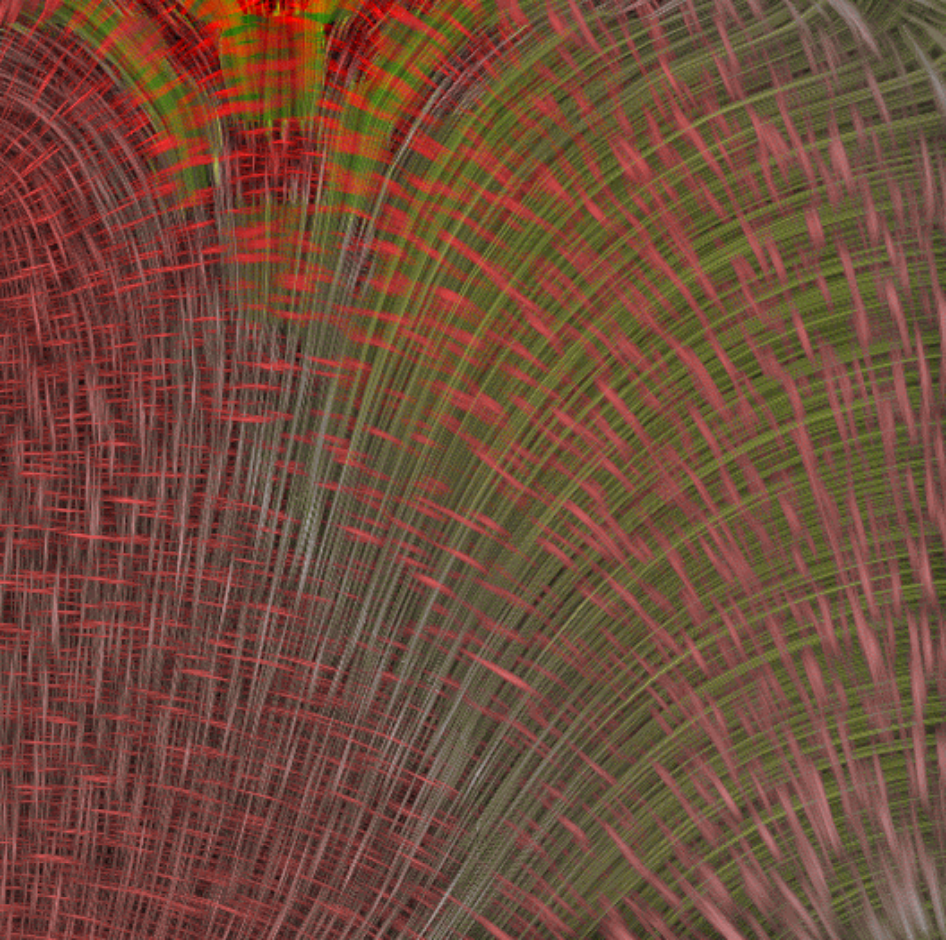
\includegraphics[width=0.6\textwidth]{figures/tensor_lic_variable_texture.png}
    \end{captionbeside}
    % \caption{LIC with variable input textures showing a stress tensor field of a
    % two point load dataset with a pushing and pulling force. Red shows negative
    % eigenvectors (compressive stress), green shows positive eigenvectors
    % (tensile stress). Density, spot size, color intensity and convolution length
    % are varied according to the local eigenvalues. Image source: Hotz
    % \etal~\cite{Hotz2004}.}
\end{figure}
%
% subsubsection lic_with_variable_input_textures (end)

\subsection{Glyph-Based Methods} % (fold)
\label{sub:tensor_glyph_based}
%
Glyph-based methods for tensor field visualization place small geometric objects
in space to represent certain characteristics of the local tensor.
%
They have the advantage of being able to display all features of a tensor at
once, but their visual complexity can make them hard to read.
%
Glyph-based methods generally differ by the restrictions they place on the
tensor.
%
There are various glyph designs for \emph{symmetric positive definite},
\emph{symmetric (indefinite)}, and \emph{general tensors} in both \ac{2D} and
\ac{3D}.
%
Some research has also focused on how to place and distribute glyphs to better
emphasize global structures in the data, as opposed to the simple regular
grid-based approach~\cite{Kindlmann2006,Feng2008}.
%

\subsubsection{Symmetric Positive Definite Tensors} % (fold)
%
Symmetric positive definite tensors are tensors that always have positive
real eigenvalues, and whose eigenvectors are orthogonal.
%
The domain most explored in scientific visualization for these tensors is
\ac{DTI} data, where they represent the diffusion of Hydrogen atoms in organic
tissue (specifically in neural fibers of the brain).
%
The simplest glyphs for visualizing such tensors are ellipses~\cite{Basser1996},
cylinders~\cite{Wiegell2000} or boxes~\cite{Schroeder2006}.
%
These glyphs are formed by placing some prototypical base shape (a unit sphere
or cube) centered at the origin and then transforming it according to the
tensor.
%
The resulting glyph is then placed at the sampling position the tensor
originated from.
%
Most often, the glyphs are also scaled to achieve a size fitting with the
glyph density.
%
Such simple glyphs accurately represent how the tensor transforms input vectors
to output vectors.
%
The disadvantage is that they have various visual ambiguities that make their
interpretability less than ideal~\cite{Kindlmann2004}.
%

%
Kindlmann~\cite{Kindlmann2004} solved this problem by carefully designing
glyphs based on superquadrics.
%
These superquadrics change their base shape depending on the relationship of
the three eigenvalues of the tensor.
%
In this way, ambiguities intrinsic to the usage of constant base shapes are
eliminated.
%

\subsubsection{Symmetric Tensors} % (fold)
%
General symmetric tensors always have real orthogonal eigenvectors, but their
eigenvalues can be negative.
%
This poses a challenge for glyph design.
%
Simply transforming a symmetric base shape with the tensor will produce the same
image for eigenvalues with equal magnitude but opposite sign.
%
Different glyphs for symmetric tensors in different application domains have
been proposed in the literature~\cite{Pajevic1999,Hashash2003,Jeremic2002}.
%
Often, color is used to indicate the sign of the eigenvalue.
%
Alternatively, the glyph base shape is modified to represent the difference
between positive and negative eigenvalues.
%
Schultz and Kindlmann~\cite{Schultz2010a} built on top of all of this work to
develop a set of superquadric-based tensor glyphs that clearly indicates
eigenvalue sign by a combination of color and concave shape (see
\cref{fig:tensor_glyphs}).
%
% \begin{figure}[t]
%     \begin{tikzpicture}
%         \node (pos) {
%             \includegraphics[width=0.3\textwidth]{figures/diffusion_tensor_glyphs.png}
%         };
%         \node[anchor=west] (symm) at (pos.east) {
%             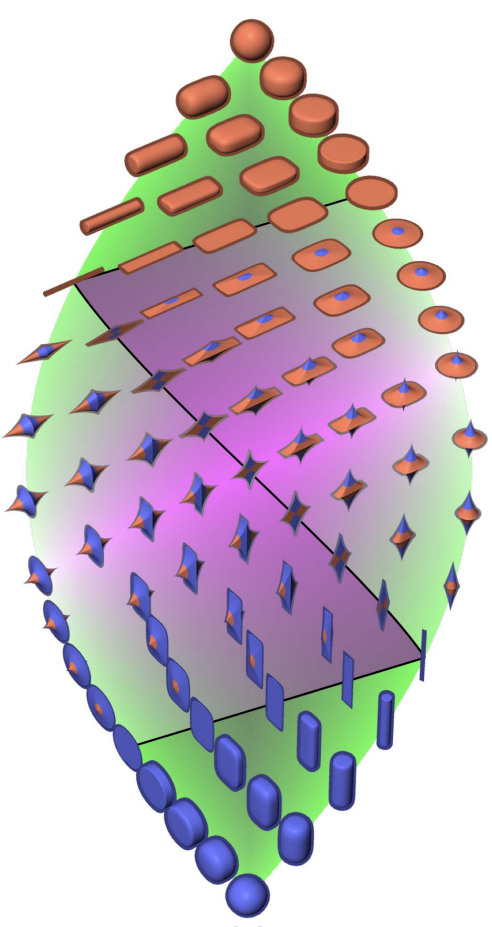
\includegraphics[width=0.3\textwidth]{figures/symmetric_tensor_glyphs.png}
%         };
%         \node[anchor=west] (general) at (symm.east) {
%             \includegraphics[width=0.3\textwidth]{figures/general_tensor_glyphs.png}
%         };
%     \end{tikzpicture}
%     \caption{Superquadric tensor glyphs for symmetric positive definite (left),
%     symmetric indefinite (middle), and general (right) tensors.}
%     \label{fig:tensor_glyphs}
% \end{figure}
%
% \begin{figure}[t]
%     \centering
%     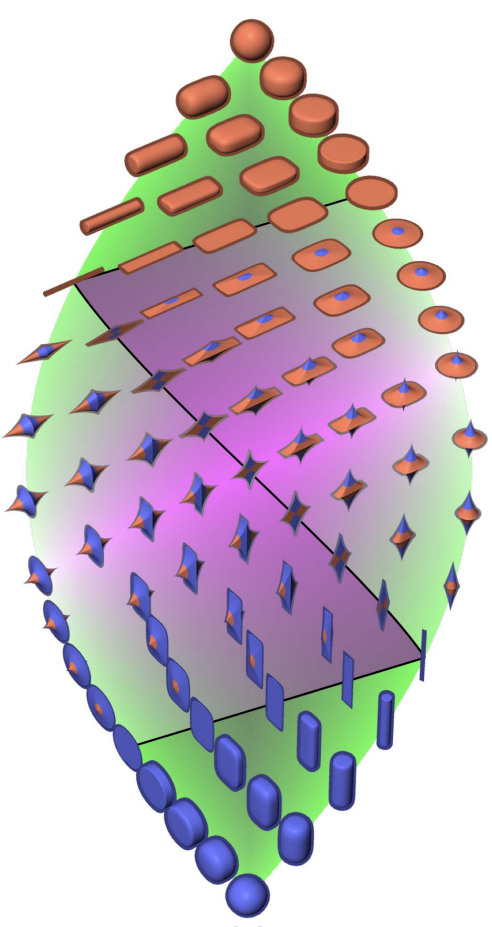
\includegraphics[width=0.5\textwidth]{figures/symmetric_tensor_glyphs.png}
%     \caption{Superquadric glyphs for symmetric tensors. Image source: Schultz
%     \etal~\cite{Schultz2010a}.}
%     \label{fig:tensor_glyphs}
% \end{figure}
%
\begin{figure}
    \begin{captionbeside}
        {Superquadric glyphs for symmetric tensors. Includes glyphs for positive
         definite tensors as a subset (top triangle). Image source: Schultz
         \etal~\cite{Schultz2010a}.\label{fig:tensor_glyphs}}
        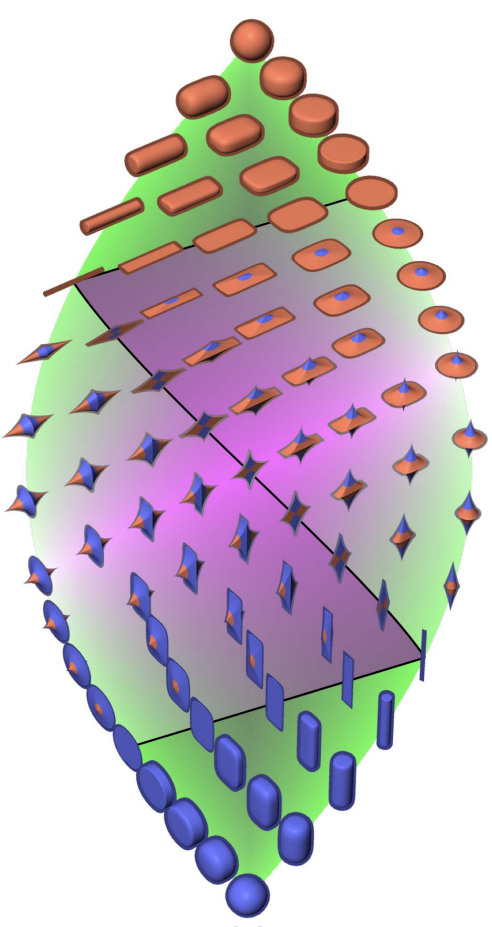
\includegraphics[width=0.4\textwidth]{figures/symmetric_tensor_glyphs.png}
    \end{captionbeside}
\end{figure}

\subsubsection{General Tensors} % (fold)
%
Apart from different eigenvalue signs, the eigenvectors of general (asymmetric)
second-order tensors need not be orthogonal, and they can be complex.
%
Gerrits \etal~\cite{Gerrits2017} built on top of the work of Kindlmann \etal to
design a set of glyphs for general tensors in \ac{2D} and \ac{3D} that can
represent non-orthogonal eigenvectors and additionally incorporates information
about complex eigenvalues via color.
%

\subsection{Line-/Surface-Based Methods} % (fold)
\label{sub:tensor_line_surface_based}
%
Line- and surface-based methods for the visualization of second-order tensor
fields are very similar to integral lines and surfaces for vector fields.
%
They work by considering the eigenvectors of the tensor field as the equivalent
of a vector field and basing the visualization on the resulting field lines.
%
Of course these methods can only visualize real eigenvectors and are therefore
generally applied to symmetric tensor fields only.
%
Because of the differences between real vector fields and eigenvector fields,
modified integration methods are necessary to form these field lines.
%
The most important methods based on this principle are \emph{tensor field
lines}, \emph{hyperstreamlines}, \emph{tensorlines} and
\emph{hyperstreamsurfaces}.
%

\subsubsection{Tensor Field Lines} % (fold)
%
\Todo{Make vocabulary consistent in tensor core lines chapter}
Tensor field lines are lines that are everywhere tangent to an eigenvector of
the tensor field.
%
They are the basis for all the methods in this category.
%
Tensor field lines have been known as \emph{stress trajectories} (see
\cref{fig:stress_trajectories}) in the context of solid mechanics since the
1800s.
%
Early stress visualizations using this technique were drawn by hand based on
photoelastic measurement techniques~\cite{Focht1962,Timoshenko1983}.
%
In a computer, these lines are obtained by integrating a vector field generated
from the eigenvector field by choosing an orientation and magnitude at each
location \cite{Dickinson1989,Tricoche2006}.
%
Since this choice is not always unique in the vicinity of degenerate points
where two or more eigenvalues are equal, special care has to be taken to avoid
a sudden flip of direction.
%
The resulting lines show the continuous change of direction of eigenvectors in
the tensor field, but they are not well suited to judge the magnitude of the
eigenvalues.
%
\begin{figure}[t]
    \centering
    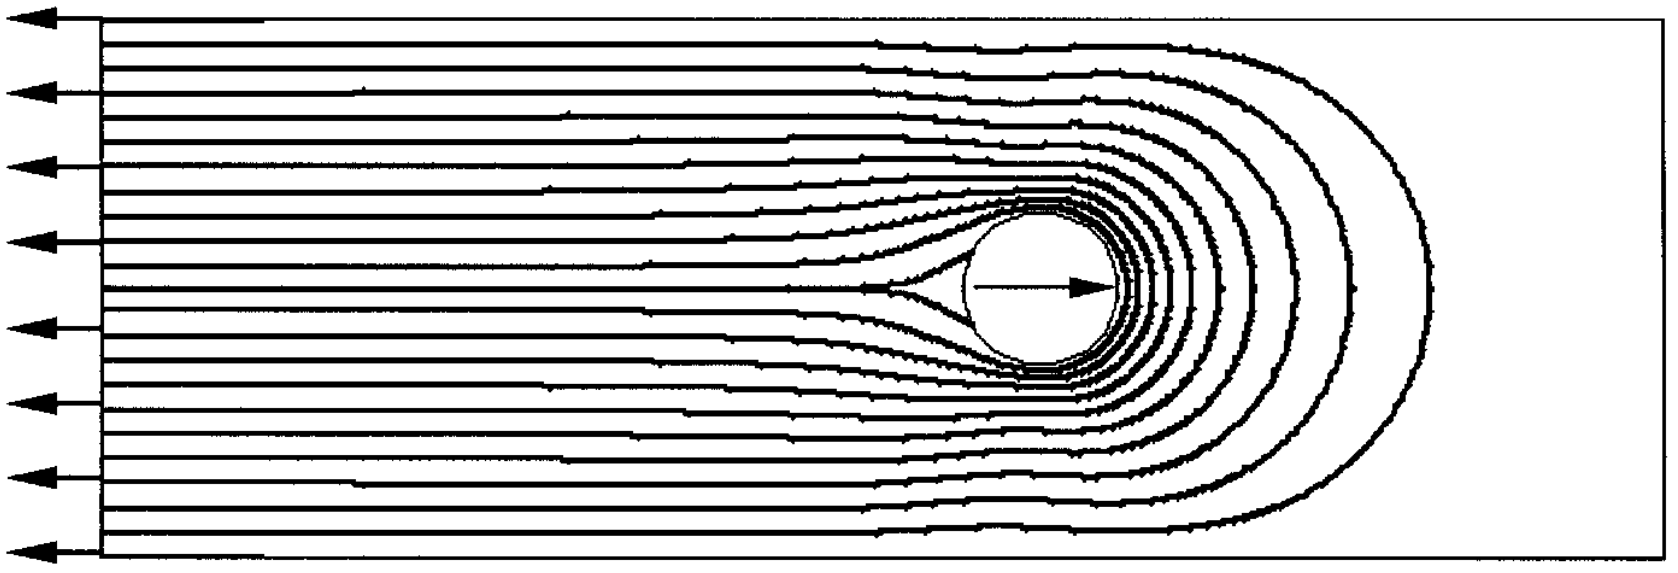
\includegraphics[width=0.8\textwidth]{figures/stress_trajectories.png}
    \caption{Major principal stress trajectories in a plate with a loaded hole.
             Image source: Kelly and Tosh~\cite{Kelly2000}.}
    \label{fig:stress_trajectories}
\end{figure}
%

\subsubsection{Hyperstreamlines} % (fold)
%
To enhance the information content of tensor field line visualizations,
Delmarcelle and Hesselink introduced hyperstreamlines~\cite{Delmarcelle1993}.
%
These hyperstreamlines follow the field lines of one of the eigenvectors of the
tensor field, while their cross-section is a cross shape or ellipse aligned with
the other two eigenvectors and scaled by the corresponding eigenvalues.
%
The eigenvalue corresponding to the eigenvector parallel to the hyperstreamline
is color-coded on the surface.
%
In this way, the full information of the tensors along the hyperstreamlines is
visualized.
%
It is important to note here that the term hyperstreamline is sometimes used
in the literature to mean what we introduced as tensor field lines.
%
In this work, we use it exclusively for lines with a variable cross-section.
%

\subsubsection{Tensorlines} % (fold)
%
In the analysis of diffusion tensor fields obtained from \ac{DTI} scans of the
human brain, tensor field lines are tracked to obtain the paths of neural
fibers.
%
Because this data suffers from noise and partial voluming effects due to limited
resolution, near-isotropic areas can occur where fibers with different
directions cross.
%
In these areas, the eigenvector direction is not clearly defined and often
dominated by noise.
%
Just following the vector field obtained from a single eigenvector will result
in random paths that do not represent the paths of actual brain fibers.
%
To counteract this problem, Weinstein \etal~\cite{Weinstein1999} introduced
tensorlines.
%
The core of the algorithm is a modified streamline integration that not only
takes into account the direction of the major eigenvector but is also guided
by the direction of the previous step in near-isotropic regions.
%

\subsubsection{Hyperstreamsurfaces} % (fold)
%
The concept of hyperstreamlines was extended to hyperstreamsurfaces by Jeremi\'c
\etal~\cite{Jeremic2002}.
%
They are formed analogous to streamsurfaces by using a curve instead of a point
as a seed structure for integration.
%
In this case, the other eigenvectors and eigenvalues can not be sensibly
displayed by varying a cross section like with hyperstreamlines.
%
Instead, only the eigenvalue of the integrated eigenvector is color-coded on the
surface.
%

\subsection{Topological Methods} % (fold)
\label{sub:tensor_topological}
%
Similar to scalar- and vector fields, topological structures in tensor fields
are defined by some mathematical degeneracy.
%
In contrast to the topology of vector fields, it is not the magnitude of the
tensor that is important, but the relationship between the eigenvalues and
eigenvectors.
%
For symmetric tensor fields, the topology is formed by \emph{degenerate points
and lines} and their \emph{separatrices}, as well as \emph{neutral and traceless
tensors}.
%
For \emph{general (asymmetric) tensor fields}, the topology is formed by
degenerate structures and circular points.
%

\subsubsection{Degenerate Points and Lines} % (fold)
%
The core of topological analysis of symmetric tensor fields are degenerate
structures.
%
These are structures where two eigenvalues are equal, and the eigenvector
directions are not uniquely defined.
%
They are the locations where tensor field lines intersect.
%
In \ac{2D} tensor fields, such structures can be classified into trisector and
wedge points, depending on the behavior of the tensor field lines in their
vicinity.
%
In \ac{3D}, degenerate features form lines.
%
Zheng \etal~\cite{Zheng2005b} showed that the type of degenerate point can
switch at isolated points along these lines.
%
These are the points where the degenerate line is parallel to the plane spanned
by the valid eigenvectors corresponding to the dual eigenvalue.
%
Degenerate lines in symmetric tensor fields were first studied by Delmarcelle,
Hesselink \etal~\cite{Delmarcelle1994,Hesselink1997}.
%
Numerical algorithms for their robust extraction were developed by Zheng
\etal~\cite{Zheng2004,Zheng2005} and later adapted for noisy \ac{DTI} data by
Tricoche \etal~\cite{Tricoche2008}.
%
\Cref{fig:tensor_topology} shows the topology of a common test case in
structural mechanics where two point loads are applied to the surface of a solid
block.
%
\begin{figure}[t]
    \begin{captionbeside}
        {Topology of the stress tensor in a double point load dataset. Image
         source: Zheng and Pang~\cite{Zheng2004}.\label{fig:tensor_topology}}[o]
        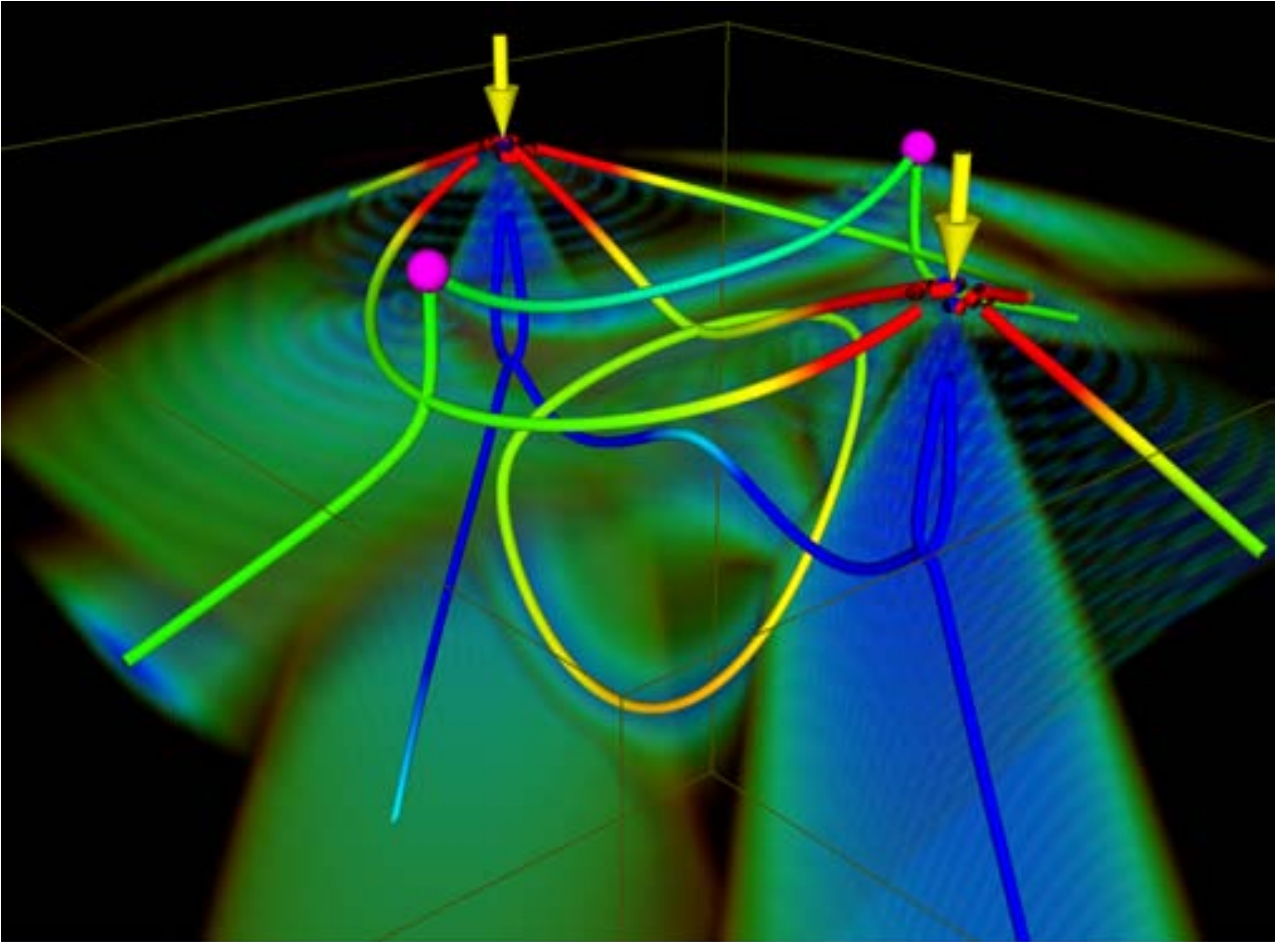
\includegraphics[width=0.6\textwidth]{figures/tensor_topology.png}
    \end{captionbeside}
\end{figure}
%

\subsubsection{Separatrices} % (fold)
%
The tensor field lines that pass through a degenerate point form separatrices
that separate the neighborhood of the point into sectors~\cite{Delmarcelle1994}.
%
These structures are akin to the separatrices of vector fields that separate
the area around a saddle point.
%
In \ac{2D}, these separatrices are lines, in \ac{3D}, they form surfaces.
%
An algorithm for extracting such surfaces from \ac{3D} tensor fields was
proposed by Zheng \etal~\cite{Zheng2005b}
%

\subsubsection{Neutral and Traceless Tensors} % (fold)
%
A different kind of topological feature are neutral and traceless tensors,
which were first investigated bu Palacios \etal~\cite{Palacios2016}.
%
A neutral tensor is a tensor where the middle eigenvalue is the average of the
major and minor eigenvalue.
%
Neutral tensors in \ac{3D} tensor fields form surfaces.
%
These surfaces mark the transition between areas of linear tensors (one
dominating eigenvalue) and planar tensors (two dominating eigenvalues).
%
In stress tensors, these can be interpreted as the transition between
predominantly tensile stress and predominantly compressive stress.
%
In diffusion tensors from \ac{DTI}, they indicate the separation between
regions with clear fiber direction and regions where fiber tracts cross.
%

%
Traceless tensors are tensors whose sum of eigenvalues is zero.
%
Traceless tensors also form surfaces in \ac{3D} tensor fields.
%
They mark the transition between areas of positive and negative trace.
%
In stress and strain tensors, these are equivalent to regions of expansion and
compression.
%
Recently, Roy \etal~\cite{Roy2019} proposed a more robust extraction method for
these surfaces as well as degenerate lines.
%

\subsubsection{Topology of General (Asymmetric) Tensor Fields} % (fold)
%
The topology of general tensor fields has been studied to a lesser extent.
%
Zheng and Pang~\cite{Zheng2005a} first introduced \emph{circular points} as the
main topological structure in \ac{2D} general tensor fields.
%
These are points where the tensor is a perfect rotation matrix.
%
Analogous to degenerate points in symmetric tensor fields, these are also points
where all vectors are valid eigenvectors.
%
Degenerate structures where two eigenvalues are equal also exist in general
tensor fields, but here they mark the transition between regions of real and
complex eigenvectors.
%
This means that they form lines instead of points in \ac{2D}, and their meaning
is very different.
%
Zhang \etal~\cite{Zhang2009} later extended the study of \ac{2D} general tensor
fields by defining eigenvector and eigenvalue manifolds to classify general
tensors and distinguish different types of circular points.
%
% subsection topological_methods (end)
%
% section tensor_fields (end)
%
% chapter fundamentals (end)